\documentclass{article}
\usepackage{graphicx}
\usepackage[
backend=biber,
style=alphabetic,
sorting=ynt
]{biblatex}
\addbibresource{sample.bib} %Import the bibliography file

\usepackage{xcolor}
\usepackage{listings}
\usepackage[hidelinks]{hyperref}
\usepackage{caption}
\usepackage{subcaption}
\usepackage{float}

\definecolor{mGreen}{rgb}{0,0.6,0}
\definecolor{mGray}{rgb}{0.5,0.5,0.5}
\definecolor{mPurple}{rgb}{0.58,0,0.82}
\definecolor{backgroundColour}{rgb}{0.95,0.95,0.92}

\lstdefinestyle{CStyle}{
    backgroundcolor=\color{backgroundColour},   
    commentstyle=\color{mGreen},
    keywordstyle=\color{magenta},
    numberstyle=\tiny\color{mGray},
    stringstyle=\color{mPurple},
    basicstyle=\footnotesize,
    breakatwhitespace=false,         
    breaklines=true,                 
    captionpos=b,                    
    keepspaces=true,                 
    numbers=left,                    
    numbersep=5pt,                  
    showspaces=false,                
    showstringspaces=false,
    showtabs=false,                  
    tabsize=2,
    language=C
}

\begin{document}
\title{Concurrent Skiplists}
\author{Thomas Fromherz (11909438)
\and
Melvin John (11905179)
\and
Christopher Hofmann (11905170)}
\maketitle

\tableofcontents

\section{Introduction}
The skiplist is a probabilistic data structure that allows both fast insertion and search. It therefore combines the advantages of balanced trees and sorted arrays. Balanced trees are great when inserted elements are randomly distributed. However there are uses cases where elements have to be inserted that are completely ordered or consist of ordered sequences (e.g. reading in names form an ordered file,...). In this cases the balanced binary tree delivers poor performance as lots of rebalancing operations are necessary. A sorted array which offers great searching performance does not allow easy insertion at all. The skiplist manages to maintain logarithmic average complexity for both operations. It is not explicitly balanced but keeps its balance probabilistically by involving a random number generator. The skiplist therefore offers similar performance as a binary tree with random insertion but does not require the insertions to be random. The author of the paper that introduced skiplist originally also claims, that the use of a random generator instead of manual rebalacning leads to simpler algorithms and therefore to a significant improvement in performance \cite{skiplist}. In the course of this project we implemented the textbook version of the skiplist as it was initially invented as well as four different concurrent versions with and without usage of locks. We were able to show the expected superiority of the lockfree implementation versus the locked implementation. Furthermore we achieved also a slight performance improvement in the lockfree version by adapting improvement suggestions from a paper about concurrent linked lists.

\section{The Idea of the Skiplist}
The main drawback of the traditional linked list is the poor searching performance. For a search in the linked list it is required to examine $n$ Nodes in the worst case, where $n$ is the number of elements in the list. If every second node had a pointer not only to the next node but also two nodes ahead this would allow us to skip every other node when traversing the list until we either reach the searched node or we overran it and have to go back by one node. Therefore only \(\lceil \frac{n}{2}\rceil +1 \) nodes need to be examined in the worst case. This idea can be extended to every \(2^i\)th node having a pointer \(2^i\) nodes ahead allowing for only \(\log_2(n)\) search steps in the worst case. However an insertion would be very tedious as all of the succeeding pointers and all pointer pointing to succeeding elements would need to be updated. In the worst case ALL additionally introduced pointers need to be updated when inserting in the beginning. William Pugh fixed this problem in 1989. He proposed to randomly choose the number of next pointers of a node upon insertion and calls a node with $k$ pointers a level $k$ node. The random distribution must be such that there are 50\% level $1$ nodes, 25\% level $2$ nodes, 12.5\% level $3$ nodes and so on. The level of a node is determined once and never changed. Now an insertion or deletion only requires local changes and can be done in constant time. As we will present in the subsequent sections this idea allows quite performant implementations not only as a sequential but also as a concurrent data structure.

\section{Implementation}
As all necessary algorithms are already known from the lecture we will only give a short overview here. Where our implementation differs from the suggested one we will of course go into more detail. \par \medskip
\noindent
The skiplist is implemented as linked list where each node stores a level $k$ and and array of $k$ forward pointers. The list at bottom level 0 represents the entire set. One important property is the sublist property: The list at level $l, l>0$ is a sublist of the list at level $l-1$. 

\subsection{Sequential Skiplist}
The sequential skiplist introduces four operations: find(x), contains(x), add(x), remove(x). \par \medskip

\noindent \textbf{find(x) and contains(x)} operate very similar. They start at the current maximum level, traverse the list at this level and keep a predecessor and current pointer. The traversal stops when pred.key $<$ x $\leq$ curr.key. Then the level is decremented and the pred and currr pointers represent the head and tail for the search at the new level. The search is successful if curr.key == x and fails if at level 0 the key has not been found. The contains operations returns a boolean whereas the find operation also returns a so-called window that contains predecessor and current pointers from each level such that pred.key $<$ x $\leq$ curr.key or NULL if the key is not found. \par \medskip

\noindent The \textbf{add(x)} operation uses the find(x) operation to check if the key is already present. If not the return value delivers the desired position of x in the list. The node can be created and linked such that for each level l it holds that pred.next[l] == new\_node and new\_node.next[l] == curr where pred and curr represent the window returned by find(x). \par \medskip

\noindent The \textbf{remove(x)} operation also relies on the find(x) operation. If successfull all pointers from the pred node returned by find(x) are set to the successor of the node to be removed. 

\subsection{Concurrent Skiplist}
The properties of the skiplist also allow for implementations that can be used in concurrent environments. There are several versions of the concurrent skiplist that mainly differ in the usage of locks and the application of more or less sophisticated optimizations. In the course of this project we implemented four versions of the concurrent skiplist wich we will regard to as \textit{locked skiplist} (a version using OpenMP locks), \textit{lockfree skiplist} (a naive lockfree implementation), \textit{improved lockfree skiplist} and \textit{predecessor lockfree skiplist} (both versions implementing optimizations suggested for concurrent linked lists in \cite{improvements}). All concurrent skiplists support the same interface as the sequential version.

\subsubsection{Locked Skiplist}
The locked skiplist introduces per-node locks to guarantee mutual-exclusiveness of the modifying operations add(x) and remove(x). In this project we used OpenMP nested locks (reentrant). The locked skiplist is a lazy implementation meaning that an element is removed by setting a marked flag. To keep the sublist property linking in must happen from the bottom to the top and linking out in the opposite direction. A node is in the list if it is contained at level 0 and it is not marked and fully linked. The latter two properties are stored inside each node. \par \medskip

\noindent The \textbf{find(x) and contains(x)} operations work the same way as in the sequential implementation. However it's worth noting that these operations are wait-free as they involve neither locks nor spinning. \par \medskip 

\noindent The \textbf{add(x)} operation again relies on the find(x) operation. However now if a node is found it must be checked if it is marked. If it not marked and fully linked the add operations returns false indicating x is already present. If a marked node is found it means it is currently being removed by some other thread. In this case we restart the add operation. Otherwise the return value of find(x) indicates the position for insertion. Now the locks of all predecessors and successors are being acquired from the bottom to the top. After acquiring a lock it must be validated that the locked node has not been marked (=removed) by some other thread. If this is the case the add operation must restart. Only after all locks have been acquired and validated the new node can be linked in from the bottom to the top. Of course all locks have to be unlocked even upon failed validation. \par \medskip

\noindent The \textbf{remove(x)} operation again first invokes the find(x) operation. If the key is found its node can either be marked or not.  If it is not marked the thread tries to lock and mark it (and store the success in a local variable). It will succeed unless another thread marks it first. In this case the remove operation aborts. If the thread finds the keys node to be marked already it will abort the operation if it has not been marked by itself (checking local success variable). Now the node can be linked out. Therefore the locks of predecessors and successors in all levels are acquired from the bottom to the top. If this succeeds, the node can be linked out from top to bottom. If one of the lock acquisitions fail the remove operations restarts (now it's important to have the local success variable indicating that the node has been marked by the thread itself). 
\medskip

\subsubsection{Lockfree Skiplist}
In order to implement a concurrent skiplist without locks we need a way to update the next pointer and marked flag at once and atomically. In our implementation we use the atomic\_compare\_exchange\_weak function from sdtatomic.h library. However this function can only handle one word at a time. Therefore from now on we store the marked flag inside the next pointer in each level. This can safely be done by using one of the upper bits of the pointer as usually only 48 of the 64 bits are used. However this is platform and implementation dependant and is therefore not recommended in general. One consequence is that we can no longer maintain the sublist property. An element is in the list if and only if it is in the list at level 0. Level $l, l > 0$ is now only a shortcut into level $l-1$.\par \medskip

\noindent The \textbf{find(x)} operation now also has to link out marked nodes. The operation starts at the top level of the head and traverses the nodes. It keeps a predecessor and current pointer. If it encounters a marked node it tries to link it out. In order to do so the thread atomically compares the next pointer of the predecessor with the current pointer and if they are identical it will update the next pointer of the predecessor to the successor of the current node (= CAS ). If the CAS operation fails it means that another thread has linked out or added a node in between and the find(x) operation restarts. The find operation continues per level until it reaches the position where x must be stored and stores the predecessor and current nodes. The predecessor node is also the starting node for the next level. In level 0 the check if the item is in the list can be done and all collected predecessor and current pointers from top to bottom are returned. \par \medskip

\noindent The \textbf{contains(x)} operation simply traverses the level 0 list and uses the upper levels as shortcuts to the bottom. If the key is found at the expected position, true is returned, otherwise false.\par \medskip

\noindent The \textbf{add(x)} operation again uses the find(x) operation to check if x is already present and aborts if it is found. Otherwise, the thread tries to link in the new node in level 0. It does so by atomically checking if the predecessor is still followed by the successor returned by the find(x) operation and updating the next pointer of the predecessor to the new node (CAS operation). The success of the CAS marks the linearization point of the add(x) because it is sufficient for an element to be contained in level 0 for it to be counted as contained in the set. If the CAS fails the add operation restarts. Otherwise the remaining levels are linked in using CAS operations, too. Upon failure of a CAS, the predecessors and successors have to be redetermined via another call to find(x). \par \medskip

\noindent The \textbf{remove(x)} operation also calls find(x) first. If the element is not found the operation aborts. Otherwise the thread starts to mark the pointers of the node to be removed starting from the top and going down to level 1. The marking is done atomically by checking if the next pointer is still the same and setting the mark from false to true. Afterwards the same is repeated for level 0 with one exception. Now it must be checked if another thread managed to mark the node first, in which case false is returned. Otherwise the operation succeeded and returns true.

\subsubsection{Improved Lockfree Skiplist}
One goal of this project also was to read and understand the paper \cite{improvements} by Träff and Pöter and try to implement the suggestions for the skiplist. The paper suggests several improvements for concurrent lockfree ordered linked lists. As the skiplist is an enhanced linked list it is reasonable to try to apply the same improvements here. We managed to apply some of the improvements in a per-level fashion, as each level can be considered a separate linked list. In this section we describe improvements applied to the add(x) and find(x) operation.\par \medskip

\noindent The first observation from the paper is, that in the case of a failed CAS operation in the \textbf{find(x)} function the search does not always have to be restarted. We managed to adapt this observation for our find(x) operation and the result can be seen in listing \ref{lst:improved_find}. If the CAS fails, we check if it failed due to a change of the marked flag or due to a change in the next pointer. If the node became marked, we still need to restart. However if only the pointer to the next node was updated, we simply update the local predecessor, current and successor pointers as well and can try the CAS operation again. 

\begin{lstlisting}[float,floatplacement=H,style=CStyle, caption=Improved find(x) operation, label=lst:improved_find]
curr = getpointer(pred->nexts[l]);
while(true){
    succ = getpointer(curr->nexts[l]);
    marked = ismarked(curr->nexts[l]);
    while(marked){
        // ------ old --------
        if(!CAS(&pred->nexts[l], &curr, succ)){
            goto _continue; //continue outer loop
        }
        // -------------------
        // ---- improved -----
        if(!CAS(&pred->nexts[l], &curr, succ)){
            if(ismarked(pred->nexts[l])){
                goto _continue; //continue outer loop
            }
        }
        curr = getpointer(pred->nexts[l]);
        succ = getpointer(curr->nexts[l]);
        marked = ismarked(curr->nexts[l]);
        // -----------------
    }
    ...
    _continue:;
}
\end{lstlisting}


\noindent The second observation by Träff and Pöter regards the \textbf{remove(x)} operation. Again upon CAS failure they suggest to check why the operation failed. If it failed because another thread marked the node to be removed, the operation aborts. Otherwise the pointer must have changed and the operation tries again with the new pointer. However we already implemented this behavior in our naive lockfree list, as it was already suggested in the lecture. We will not deal with this improvement in this report. \medskip

\noindent The third improvements suggestion regards the \textbf{add(x)} operation. Träff and Pöter found that upon a failed CAS when trying to update the next pointer of a node again two cases must be considered. Either the CAS failed because the node became marked. In this case we need to repeat the find(x) operation. However if the CAS failed because a pointer changed (=another node has been inserted), it is sufficient to continue searching for the new spot starting from the current spot. The implementation can be seen in listing \ref{lst:improved_add}.

\begin{lstlisting}[float,floatplacement=H,style=CStyle, caption=Improved add(x) operation, label=lst:improved_add]
pred = preds[0];
succ = getpointer(succs[0]);
// ------ old --------------
if(!CAS_improved(&pred->nexts[0], &succ, new_node)){
    continue; // restart entire operation including find(x)
}
// --------------------------

// ----- improved -----------
while(!CAS(&pred->nexts[0], &succ, new_node)){
    if(ismarked(pred->nexts[0])){
        goto restart_1; // restart entire operation including find(x)
    }
    succ = getpointer(pred->nexts[0]);
    while(succ->key < new_node->key){
        pred = succ;
        succ = succ->nexts[0];
    }
    new_node->nexts[0] = succ;
}
// -------------------------
\end{lstlisting}

\subsubsection{Predecessor Lockfree Skiplist}
In \cite{improvements} Träff and Pöter also suggested introducing predecessor pointers for each node. This improvement allows us to prevent to restart an operation even if a CAS failed because of a node getting marked. In this case we can indicate the search function to go back to an unmarked node and restart the search from there. We implemented this improvement by using $l$ predecessor pointers for each node, where $l$ is the level of the node. \medskip

\noindent
The \textbf{find(x)} operation now takes as an input also an array of predecessor pointers which serve as a shortcut into the last unmarked position. The operation now starts searching from there if the array is not null.  \medskip 

\noindent
The \textbf{add(x)} operation stores the position of the last unmarked node in a temp variable. Upon a CAS failing because a node got marked, the operation still restarts. However this time it will indicate the find(x) function to start from the position stored in the temp variable. The predecessor pointers from the new node to be inserted are initialized to the predecessors found in the find(x) method. \medskip

\noindent
The \textbf{remove(x)} operation does not take advantage of the predecessor pointers but simply updates them when needed.



\section{Results}
\subsection{Test Setup}
The test setup for benchmarking the different skip list implementations involves some assumptions about the typical use case of such data structures.
For the benchmarking of throughput (successful operations per second) a random mix test was constructed.
The test will perform a random iteration of add, remove and contains operations, with random keys, according to a defined ratio of these operations, e.g. 25\% adds, 25\% removes and 50\% contains.
Furthermore, the test has parameters for defining the number of operations to be performed, the max level for the lists as well as the number of threads used for the test.
The test performs the same operations on every implementation and measures the time it takes to calculate the achieved throughput.

One assumption that was made is that operations happen completely randomly, while the typical use would probably contain some patterns.
These might include longer sequences of only add operations, or sequences of alternating contains and adds or contains and removes.
Another assumption made was that keys are random, although adds often happen in sequences with increasing keys.
For the sake of benchmarking the range of randomly generated keys is restricted to $10\times\#operations$.
This was done to increase the chance that one key can occur more than once.
One other thing done to improve the representation of the typical use case was the prefilling of the lists.
This increases the chance of remove operations actually succeeding.
The lists are prefilled with $\frac{\#operations}{10}$ nodes to provide a non-empty starting point.
The test was designed in this way to get an broad look of how the different skip list implementations perform for a mix of operations while not being too specific in the test cases.

\subsection{\emph{small-bench} Benchmark}
For the \emph{small-bench} benchmark run (executed using \texttt{make small-bench}) the random mix test is performed a number of times with different parameters.
Each configuration is repeated three times for which the average throughput is taken and saved.
The configurations are as follows:
\begin{itemize}
    \item 10\% adds, 10\% removes, 80\% contains with max-level 3
    \item 25\% adds, 25\% removes, 50\% contains with max-level 3
    \item 25\% adds, 25\% removes, 50\% contains with max-level 5
    \item 25\% adds, 25\% removes, 50\% contains with max-level 10
\end{itemize}
Each is run with 16000 operations and a number of threads $2^i$ from $i=0$ to $i=6$.
This setup was chosen to provide a wide range of data and configurations while adhering to the one minute time limit on the \emph{nebula} test system.
The gathered data allows us to examine different amounts of update operations (adds/removes) and different values for max-level, while seeing how these scale with more threads.
Note that performance counters shall be disabled when executing the benchmark to gather accurate data.
In particular the lock free skip list versions suffer a big performance hit when the counters are enabled.

\subsection{Interpretation of Results - max level}
The most important part before investigating the results for the different implementations is to find a common ground. The common ground in this case would be the max level for the skip lists. We ran tests for all the implementations with three different levels: 3, 5 and 10. In Fig. \ref{fig:seq_levels} we are able to see that depending on which level we set, the performance drastically changes with the corresponding number of threads. The most stable performance for all different variations of number of threads for the sequential version is achieved by setting the level to 3 as the results show. Even though the results for the locked version in Fig. \ref{fig:lock_levels} and the lockfree versions in Fig. \ref{fig:lfree_levels} and Fig. \ref{fig:lfree_improved_levels} show performance increases with a higher max level, we decided to use level 3 for the remaining results because of said stable performance for the sequential version. In Fig. \ref{fig:lfree_pred_levels} we also see similar results for the third variation of the lockfree list. 

\begin{figure}[H]
    \centering
    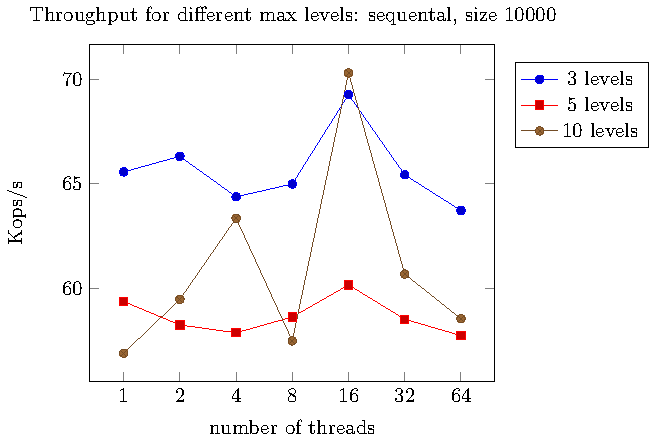
\includegraphics[width=\textwidth]{plots_for_report/seq_levels_plot.pdf}
    \caption{Sequential throughput for different max levels}
    \label{fig:seq_levels}
\end{figure}
\begin{figure}[H]
    \centering
    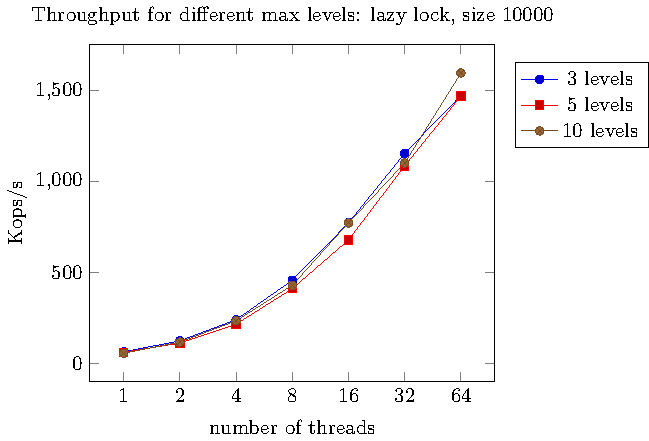
\includegraphics[width=\textwidth]{plots_for_report/lock_levels_plot.pdf}
    \caption{Lock based throughput for different max levels}
    \label{fig:lock_levels}
\end{figure}
\begin{figure}[H]
    \centering
    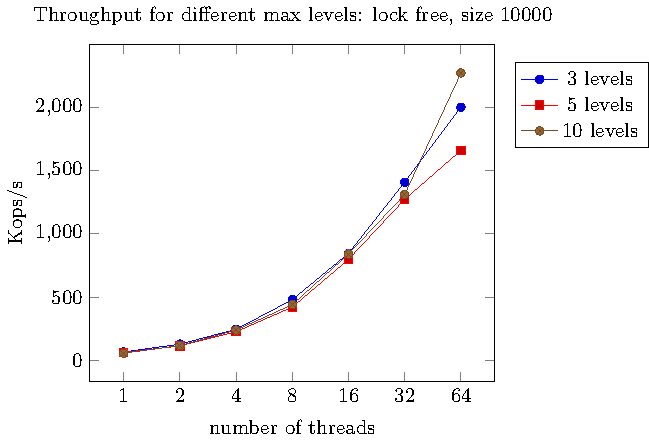
\includegraphics[width=\textwidth]{plots_for_report/lfree_levels_plot.pdf}
    \caption{Lock free throughput for different max levels}
    \label{fig:lfree_levels}
\end{figure}
\begin{figure}[H]
    \centering
    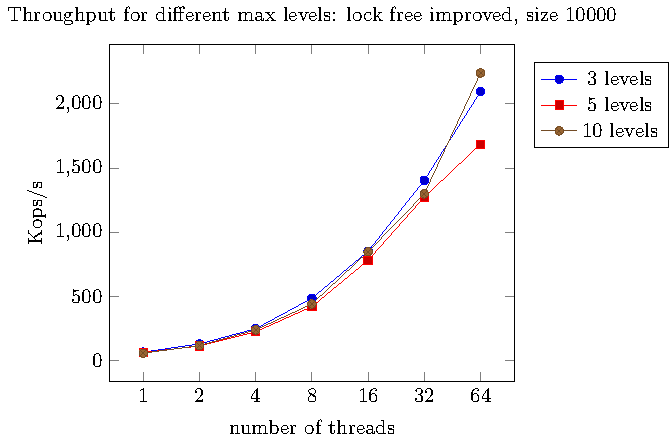
\includegraphics[width=\textwidth]{plots_for_report/lfree_improved_levels_plot.pdf}
    \caption{Improved lock free throughput for different max levels}
    \label{fig:lfree_improved_levels}
\end{figure}
\begin{figure}[H]
    \centering
    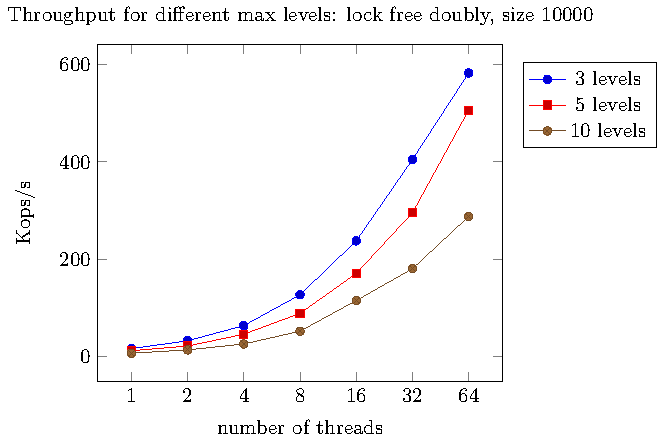
\includegraphics[width=\textwidth]{plots_for_report/lfree_pred_levels_plot.pdf}
    \caption{Lock free with predecessor throughput for different max levels}
    \label{fig:lfree_pred_levels}
\end{figure}

\subsection{Interpretation of Results with level 3}
From Figure~\ref{fig:throughput_all} it is clear that both the lazy lock based as well as the lock free skip list have a sizable absolute speed up over the baseline sequential implementation.
\begin{figure}[ht!]
  \centering
  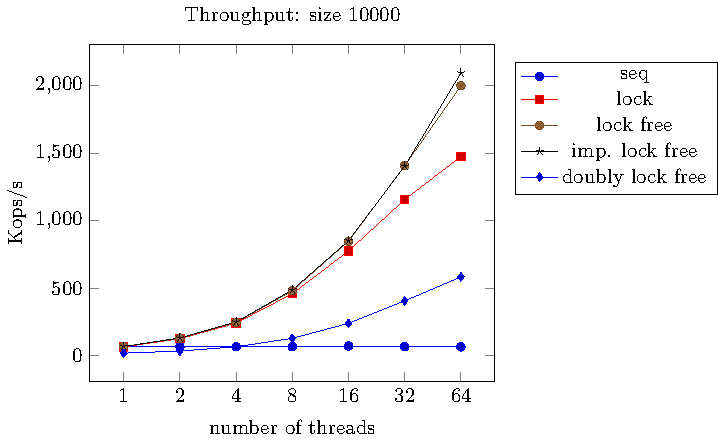
\includegraphics[width=\textwidth]{plots_for_report/throughput_plot.pdf}
  \caption{Throughput scaling of all implementations using max-level 3}
  \label{fig:throughput_all}
\end{figure}
The lock free version shows better scaling than the lock version, providing higher throughput at higher thread counts.
The improved lock free skip list only shows a slight gain in scalability.
However, due it not having any downsides, using it instead of the textbook implementation is preferred.
A regression in performance was observed from the lock free list with additional predecessor pointer.

When comparing the throughput of the sequential, lock based and textbook lock free version for two different usage scenarios, less update operations show better scaling.
Figure~\ref{fig:throughput_percent} presents the results from benchmarking two scenarios: One with 25\% adds and removes each, and one with 10\% adds and removes each.
\begin{figure}[H]
  \centering
  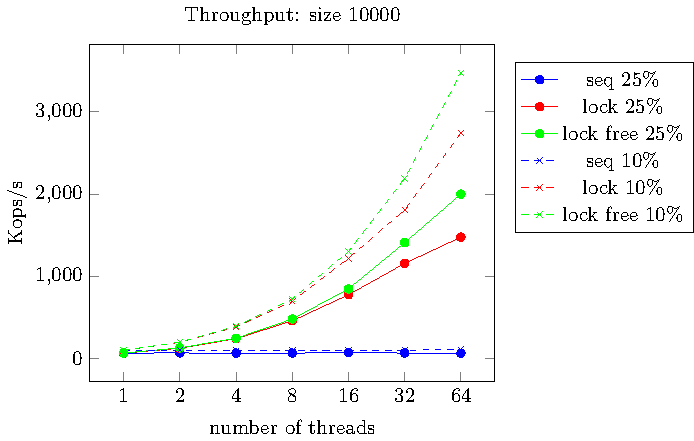
\includegraphics{plots_for_report/throughput_percent_plot.pdf}
  \caption{Throughput scaling off different ratios of update operations; max-level 3 with 25-25-50 and 10-10-80 (adds,removes,contains) ratios}
  \label{fig:throughput_percent}
\end{figure}
The better scaling of lock based and lock free variations with less update operations is not surprising considering these are the operations which need extra mechanisms for concurrent operation.
A higher ratio leads to more failed CAS operations and spinning.


\subsection{Python Global Interpreter Lock}
As stated in \cite{python_lock} all threads that are created from C do not hold the global interpreter lock. The python template calls our C function and then the threads are created. Therefore it does not interfere with with the results.







\section{Conclusion}
With the results discussed in the sections before we can guarantee a big improvement when using the concurrent skip list. We were also able to transfer some results achieved in \cite{improvements} to the concurrent skiplist. All the minor improvements converted well and a slight improvement could be measured. However, the suggestion to introduce a predecessor to the nodes failed in comparison. We lost about 70\% of the performance in the predecessor variant. In the paper a last improvement was mentioned where a cursor should be saved by threads to then start from there in the find function. For the cursor to be implemented we would need predecessor nodes in case the cursor is marked. Because of the not ideal results achieved in the predecessor variant we as a team decided that even with the introduction of a cursor, the new variant could probably not compensate a 70\% loss in performance. The biggest downside for all the concurrent implementations is the memory reclamation problem, which restricts the real world use cases. 

\newpage

\printbibliography

\end{document}